\subsubsection{Aufbau des Plugins}

Das Plugin kann in drei Hauptkomponente aufgeteilt werden:

\begin{itemize}
  \item \textbf{Plugin API:} Bildet die Schnittstelle zwischen der Capacitor Anwendung und dem Capacitor-BrowserView Plugin.
  \item \textbf{Implementierung:} Zuständig für das Erstellen und Steuern von WebViews sowie für die Kommunikation zu geladenen Webinhalten.
  \item \textbf{WebView:}
  Verantwortlich für das Anzeigen von Webinhalten auf der Benutzeroberfläche.
  Dieser Teil wird von der jeweiligen Plattform zur Verfügung gestellt.
  \cite{android:api, ios:api, electron:docs}
\end{itemize}

\begin{figure}[H]
  \centering
  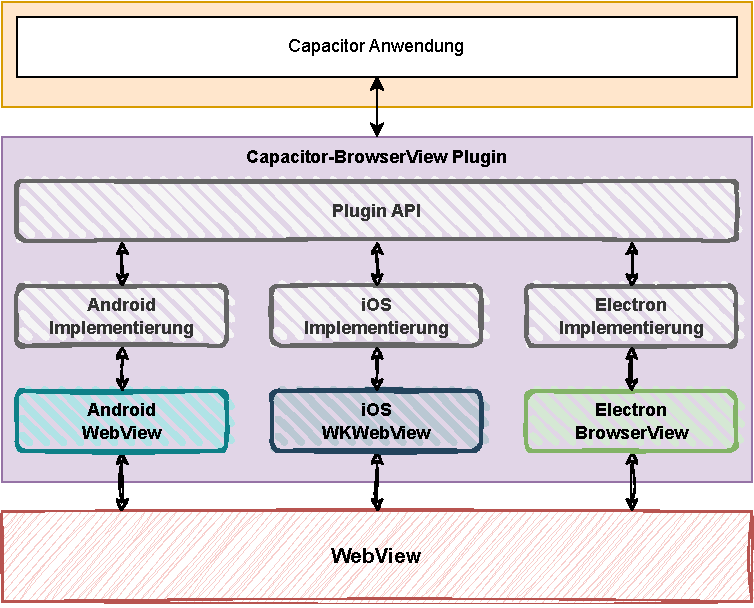
\includegraphics[width=\textwidth]{assets/03_Capacitor-BrowserView/02_Aufbau.drawio.pdf}
  \caption[Capacitor-BrowserView / Aufbau]{Aufbau des Capacitor-BrowserView Plugins}
\end{figure}
